\section{Interface refinement and information ordering}
\label{sec:refinement}

Different instruments or representational procedures may observe the same world at different resolutions. Interface refinement is a preorder on interfaces. Identifying mutually refining interfaces gives an order on the corresponding classes. This resembles comparison of statistical experiments by informativeness, but the present relation is deterministic and is defined by an explicit commuting coarsening map rather than by a Markov kernel or decision-risk criterion \parencite{Blackwell1951,Blackwell1953,Torgersen1991}.

Let
\[
F=(O_F,\pi_F)
\qquad\text{and}\qquad
C=(O_C,\pi_C)
\]
be interfaces on the same world state space \(X\).

\begin{definition}[Interface refinement]
The interface \(F\) refines \(C\), written
\[
F\succeq C,
\]
when there exists a coarsening map \(c:O_F\to O_C\) such that
\[
\pi_C=c\circ\pi_F.
\]
\end{definition}
The commuting equation states that every coarse observation is determined by a set function of the fine observation. It does not state that the fine observation can be recovered from the coarse observation.

\begin{proposition}[Refinement is reflexive and transitive]
Every interface refines itself. If \(F\succeq M\) and \(M\succeq C\), then \(F\succeq C\).
\end{proposition}

\begin{proof}
Reflexivity uses the identity map on \(O_F\). For transitivity, let \(a:O_F\to O_M\) and \(b:O_M\to O_C\) witness the two refinements. Then
\[
\pi_C=b\circ\pi_M=b\circ a\circ\pi_F,
\]
so \(b\circ a\) witnesses \(F\succeq C\).
\end{proof}
\subsection{Monotonicity of accessible structure}

Refinement orders observational equivalence in the expected direction.

\begin{theorem}[Fine equivalence implies coarse equivalence]
If \(F\succeq C\) and \(x\sim_F y\), then \(x\sim_C y\).
\end{theorem}

\begin{proof}
Let \(c\) witness the refinement. The equality \(\pi_F(x)=\pi_F(y)\) implies
\[
c(\pi_F(x))=c(\pi_F(y)).
\]
Using \(\pi_C=c\circ\pi_F\), this becomes \(\pi_C(x)=\pi_C(y)\).
\end{proof}
The converse need not hold. A coarse interface may identify states that a fine interface distinguishes.

\begin{theorem}[Factorization is monotone under refinement]
If \(F\succeq C\) and \(q:X\to V\) factors through \(C\), then \(q\) factors through \(F\).
\end{theorem}

\begin{proof}
Let \(q=\bar q_C\circ\pi_C\) and \(\pi_C=c\circ\pi_F\). Then
\[
q
=\bar q_C\circ c\circ\pi_F.
\]
Thus \(q\) factors through \(F\) by the map \(\bar q_F=\bar q_C\circ c\).
\end{proof}
Every coarse test can therefore be simulated from the fine observation. Exact reconstruction also moves in the same direction.

\begin{proposition}[A coarse decoder induces a fine decoder]
If \(F\succeq C\) and \(C\) has a globally exact decoder, then \(F\) has a globally exact decoder.
\end{proposition}

\begin{proof}
Let \(d_C:O_C\to X\) satisfy \(d_C\circ\pi_C=\id_X\), and let \(c:O_F\to O_C\) witness refinement. Define \(d_F=d_C\circ c\). Then
\[
d_F\circ\pi_F
=d_C\circ c\circ\pi_F
=d_C\circ\pi_C
=\id_X.
\]
\end{proof}
The contrapositive is useful: if the fine interface is noninjective, then no coarsening can be injective. Coarsening cannot restore a distinction that has already disappeared.

\subsection{Refinement maps between observable quotients}

Refinement induces a map between observable quotients.

\begin{figure}[tbp]
\centering
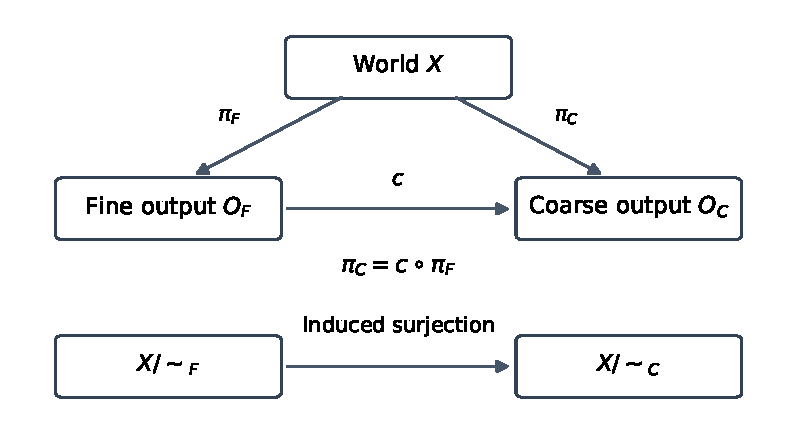
\includegraphics[width=0.88\textwidth]{figures/concept_interface_refinement.pdf}
\caption{Interface refinement and induced quotient map. The coarsening map makes the observation triangle commute. The induced map sends each fine observational class to its coarse class. The map is always surjective. Under strict refinement it is not injective.}
\label{fig:refinementdiagram}
\end{figure}

\begin{definition}[Induced quotient map]
If \(F\succeq C\), define
\[
Q_{F\to C}:X/{\sim_F}\longrightarrow X/{\sim_C}
\]
by
\[
Q_{F\to C}([x]_F)=[x]_C.
\]
\end{definition}
The map is well defined because fine equivalence implies coarse equivalence.

\begin{theorem}[Surjectivity of the quotient map]
For every refinement \(F\succeq C\), the map \(Q_{F\to C}\) is surjective.
\end{theorem}

\begin{proof}
Let \([x]_C\) be any coarse class. The fine class \([x]_F\) maps to it by definition:
\[
Q_{F\to C}([x]_F)=[x]_C.
\]
Therefore every coarse class has a fine preimage.
\end{proof}
\begin{definition}[Strict refinement]
The refinement \(F\succeq C\) is strict when there exist \(x,y\in X\) such that
\[
\pi_F(x)\neq\pi_F(y)
\qquad\text{and}\qquad
\pi_C(x)=\pi_C(y).
\]
\end{definition}
A strict refinement preserves at least one distinction that the coarse interface removes.

\begin{theorem}[Strict refinement makes the quotient map noninjective]
If \(F\) strictly refines \(C\), then \(Q_{F\to C}\) is not injective.
\end{theorem}

\begin{proof}
Choose \(x,y\) witnessing strictness. Since \(\pi_F(x)\neq\pi_F(y)\), the fine classes are distinct:
\[
[x]_F\neq[y]_F.
\]
Since \(\pi_C(x)=\pi_C(y)\), the coarse classes are equal. Hence
\[
Q_{F\to C}([x]_F)=[x]_C=[y]_C=Q_{F\to C}([y]_F),
\]
so the quotient map is noninjective.
\end{proof}
\begin{theorem}[Strict refinement prevents reverse refinement]
If \(F\) strictly refines \(C\), then \(C\) does not refine \(F\).
\end{theorem}

\begin{proof}
Suppose that \(C\succeq F\). Fine equivalence would then follow from coarse equivalence. The strictness witnesses satisfy \(x\sim_C y\) but \(x\not\sim_F y\), which is a contradiction.
\end{proof}
\subsection{Equal observational resolution}

Two interfaces can use different observation labels while preserving exactly the same partition of \(X\).

\begin{definition}[Same observational resolution]
Interfaces \(I\) and \(J\) have the same observational resolution when
\[
x\sim_I y
\quad\Longleftrightarrow\quad
x\sim_J y
\]
for every \(x,y\in X\).
\end{definition}
Mutual refinement implies equal observational resolution. Conversely, on reachable observations, equal resolution supplies mutually compatible class maps. The induced quotient maps are bijections.

\begin{theorem}[Mutual refinement gives quotient equivalence]
If \(I\succeq J\) and \(J\succeq I\), then the induced quotient maps are inverse bijections. Thus the two interfaces retain the same observational distinctions even when their observation representations differ.
\end{theorem}
This distinction separates strict coarsening from relabeling. Strict coarsening changes the partition of the world. Relabeling changes the symbols used for the classes but preserves the classes themselves.
